\documentclass{article}
\usepackage[utf8]{inputenc}
\usepackage{tkz-euclide}
\usepackage{graphicx}
\usepackage{hyperref}
\usepackage{amsmath}
\usepackage{amssymb}
\usepackage{tikz}
\usetkzobj{all}
\usepackage{verbatimbox}


\usepackage{geometry}
 \geometry{
 a4paper,
 left=15mm,
 right=10mm,
 top=20mm,
 bottom=20mm,
 }



\begin{document}



\subsection*{Reducción de las imagenes}
\begin{itemize}
\item
Separar las imagenes en carpetas por tipo: object y flat y cada una por el fitro(B, R, V) (función initDirs() in red.py)
Las nueva carpeta donde se van a poner las imagenes se llama M37New (con eso me refiero mas adelante para especificar la carpeta raiz que contiene todas las carpetas con imagenes clasificadas por tipo y filtro y a veces tiene la ruta absoluta)
\item
Correción bias(sustraer bias de la imagen): con la función colbias de iraf(función trimAndOverscan() in red.py): se calcula una columna como media de las columnas definidas en la sección bias y se sustrae de todas las columnas de la sección trim. Se hace para todas las imagenes: flat y object
\item 
Crear los ficheros flat que se usan para la correción de flat:
con imcombine se hace una media de todas las imaganes flat para cada filtro y despues se normalizan dividiendo por la media(mean) de cada uno (usando la función iraf imarith) (función createFlatFiles() en red.py)
\item
Correción de flat:
Todas las imagenes tipo object se dividen con el flat medio normalizado para cada filtro (función flatCorrection() en red.py)

\item corregir pixeles malos (independientes del filtro):
de forma aproximadamente automática: elegimos 2 flat con tiempo de exposition largo (EXPTIME keyword in header)
M37New/flat/V/Nov30032.fits (60) y M37New/flat/R/Nov30031.fits (35) y hacemos la media con imcombine
y 2 con el valor  EXPTIME pequeño: M37New/flat/V/Nov30016.fits (2)  M37New/flat/V/Nov30015.fits (2)
Luego dividimos los 2 resultados y creamos una mascara con ccdmask. Despues ejecutamos fixpix para lodas las imagenes tipo object y el fichero mask obtenido antes:

\begin{verbnobox}[\small]

ecl> imcombine M37New/flat/R/Nov30031.fits,M37New/flat/V/Nov30032.fits M37New/flat/FlatBigExptime
ecl> imcombine M37New/flat/V/Nov30016.fits,M37New/flat/V/Nov30015.fits M37New/flat/FlatSmallExptime
ecl> imarith  M37New/flat/FlatBigExptime /  M37New/flat/FlatSmallExptime  M37New/flat/FlatBigSmallDivided
ecl> noao
noao> imred
imred> ccdred
ccdred> ccdmask  M37New/flat/FlatBigSmallDivided  M37New/flat/MaskFile 
ccdred> cd M37New/object/V
ccdred> fixpix @list /scratch1/tobs/M37New/flat/MaskFile
ccdred> cd ../R
ccdred> fixpix @list /scratch1/tobs/M37New/flat/MaskFile
ccdred> cd ../B
ccdred> fixpix @list /scratch1/tobs/M37New/flat/MaskFile


\end{verbnobox}

\item Si queremos definir una mascara:

Si miramos en la imagen  Nov30098.fits y queremos definir en la columna 577($ x \in [577,578) $) como pixeles malos la parte de abajo ($ y \in [0, 259) $)
\begin{verbatim}
bpopescu@colibri:/scratch1/tobs$ cat col577Mask 
box 577 0 578 259
\end{verbatim}

\begin{verbatim}
ecl> mskregions.regions="col577Mask"
ecl> mskregions.dims="1024,1024"
ecl> mskregions.masks="M37New/flat/Col577Mask"
ecl> mskregions.refimages="M37New/object/V/Nov30098.fits"
ecl> mskregions
The list of region specifications (col577Mask): 
The list of output mask images (M37New/flat/Col577Mask): 
The list of input reference images (M37New/object/V/Nov30098.fits): 
Creating mask M37New/flat/Col577Mask.pl using reference image M37New/object/V/Nov30098.fits
    Using regions file col577Mask
ecl> 
\end{verbatim}
(Si no queremos que nos pregunte siempre por los parametros hay que modificar el parametro mode del task de 'ql' a 'h')

Se crea un fichero /scratch1/tobs/M37New/flat/Col577Mask.pl, no hace falta especificar la extensión .pl en el paso siguiente cuando se pasa como parametro al task fixpix:

Después hay que modificar todas las imagenes tipo object con fixpix como antes


\begin{verbatim}
ecl> cd M37New/object/V
ecl> fixpix @list /scratch1/tobs/M37New/flat/Col577Mask
ecl> cd ../R
ecl> fixpix @list /scratch1/tobs/M37New/flat/Col577Mask
ecl> cd ../B
ecl> fixpix @list /scratch1/tobs/M37New/flat/Col577Mask
\end{verbatim}

Miramos la diferencia entre las imagenes antes de aplicar esta mascara y despues:
			
\begin{verbatim}

        cl> display.xsize=0.5
        cl> display M37New/object/V/Nov30098.fits fill+ xcen=0.25
        cl> display Nov30098.fits erase- fill+ xcen=0.75


\end{verbatim}

\begin{figure}[!ht]
 \centering
 \includegraphics[scale=0.5]{fixpix.png}
 \caption{\emph{Perfil radial de las estrellas de referencia para la alineación}}
\end{figure}


\end{itemize}

\subsection*{Fotometría}
\begin{itemize}
\item para la fotometría elegimos solo la parte central del cúmulo (las imagenes que tienen los últimos 3 dígitos antes de la extensión .fits  formando un número $ \in  [96,105] $)
\item
\textbf{Alinear las imagenes:}
Se elige una imagen con buena respuesta(del centro del cúnulo): elegí Nov30098.fits en filtro V y 3 estrellas bien separadas en la imagen que no tengan mucho ruido y que no estén saturadas

\begin{figure}[!ht]
 \centering
 \includegraphics[scale=0.2]{align_rp.png}
 \caption{\emph{Perfil radial de las estrellas de referencia para la alineación}}
\end{figure}

\begin{verbatim}
para ver el perfil radial:
en xgterm abrir el visualizador ds9 (funciona con ximtool, pero no he probado)
en iraf
 ecl>display image.fits
 ecl>imexam image.fits
hacer click en el punto donde quieres ver el perfil radial y pulsar "r" después
\end{verbatim}


\item  escribir las coordenadas en un fichero
\begin{verbatim}
[bpopescu@colibri tobs]$ cat coords-98.txt
194 872
831 843
222 98
\end{verbatim}

\item Usamos imcentroid para obtener las coordenadas exactas usando como input la misma imagen de referencia

\begin{verbatim}

ecl> imcentroid.input = "M37New/object/V/Nov30098.fits" 
ecl> imcentroid.reference = "M37New/object/V/Nov30098.fits" 
ecl> imcentroid.coords = "coords-98.txt"
ecl> imcentroid

salen las coordenadas:

#Coords        Image     X-center   Err      Y-center   Err     Num
/scratch/M37New/object/V/Nov30098.fits     194.519 (0.028)     872.795 (0.024)     1
/scratch/M37New/object/V/Nov30098.fits     830.926 (0.015)     843.310 (0.010)     2
/scratch/M37New/object/V/Nov30098.fits     222.031 (0.018)      97.730 (0.019)     3

#Refcoords Reference     X-center   Err      Y-center   Err     Num
/scratch/M37New/object/V/Nov30098.fits     194.519 (0.028)     872.795 (0.024)     1
/scratch/M37New/object/V/Nov30098.fits     830.926 (0.015)     843.310 (0.010)     2
/scratch/M37New/object/V/Nov30098.fits     222.031 (0.018)      97.730 (0.019)     3

#Shifts        Image    X-shift   Err      Y-shift   Err      N      Internal
/scratch/M37New/object/V/Nov30098.fits      0.000 (0.017)      0.000 (0.015)    3   (0.000,0.000)

miramos los nuevos valores de x-center y y-center y los ponemos en otro fichero:

[bpopescu@colibri tobs]$ cat coords-98-aligned.txt 
194.519 872.795
830.926 843.310
222.031 97.730


\end{verbatim}

\item Alinear lodas las imagenes: usando imalign
Creamos una lista(fichero listCenter-M37) con las imagenes  que hay que alinear(las tipo "object" del centro del cúmulo (con el numero del nombre  de 96 a 105)) y otra a cual añadimos 'a' antes de la extensión (fichero listCenterAligned-M37) con createListAlignObject.py (ejecutando align desde pyraf, sale un error, porque?)

\begin{verbatim}
 	ecl>imalign.input="@listCenter-M37"   
  ecl>imalign.reference = "M37New/object/V/Nov30098.fits" 
  ecl>imalign.coords = "coords-98-aligned.txt" 
  ecl>imalign.output = "@listCenterAligned-M37" 
  ecl>imalign.interp_type = "nearest" 
	ecl>imalign
\end{verbatim}

\item  \textbf{Buscar estrellas y obtener las magnitudes}
Para poder tener valores de las medias de sky sigma y fwhm para cada imagenes (que usamo después como parametros de entrada en daofind para que busque de forma automática todas las estrellas de la imagen) cogemos algunas estrellas de referencia de  cada imagen miramos la distribucion radial de la luz = COUNTS(XCENTER, YCENTER, Rmax) de cuales queremos que iraf calcule sky sigma, fwhm y magnitud. Nos interesan sky sigma y fwhm que definen el perfil de intensidad (intenta a ajustarlo a una gaussiana con estos parámetros)

\begin{verbatim}

ecl> noao
noao> digiphot
digiphot> daophot


daophot> display M37New/object/R/Nov30103a.fits
frame to be written into (1:16) (2): 
z1=8.931553 z2=90.34003
daophot> daoedit M37New/object/R/Nov30103a.fits
despues con el cursor encima de la estrella (en la ventana ds9)(las coordenadas donde está el cursor posicionado son XCENTER y YCENTER) pulsamos 'a' y en la terminal xgterm aparece una linea para cada estrella
con las columnas :
# XCENTER YCENTER       SKY SKYSIGMA    FWHM   COUNTS     MAG
despues de seleccionar varias guardamos la salida en un fichero:
bpopescu@colibri:/scratch1/tobs$ cat M37New/object/R/Nov30103a.fits-daoedit 
# XCENTER YCENTER       SKY SKYSIGMA    FWHM   COUNTS     MAG
   832.83  575.81      43.9     6.99    4.98  54017.2 -11.831
   418.22  684.58      55.5    12.89    5.05 235331.5 -13.429
   175.20  652.63      51.5     9.59    5.04 266379.4 -13.564
    52.98  456.31      40.7     6.49    4.44  58369.4 -11.915
    89.85  235.86      47.8     9.12    4.97 211897.9 -13.315
   624.22  843.96      47.2     8.37    5.02 162999.8 -13.030
   193.41  872.61      39.7     6.35    4.88  64339.4 -12.021
   273.99  859.73      37.5     6.56    4.97  22932.2 -10.901
   348.81  133.11      46.2     9.01    5.29 153856.1 -12.968
   611.49  559.89      47.6     8.17    5.07  58278.2 -11.914
   912.48  143.12      40.0     6.54    5.62  34869.5 -11.356

Para salir de daoedit pulsamos 'q'

\end{verbatim}

\item 
Para hacer una media de las columnas 4(SKYSIGMA) y 5(FWHM) de cada fichero daoedit podemos ejecutar:

\begin{verbatim}
python daoeditAvg.py M37New/object/R/Nov30103a.fits-daoedit
sky sigma mean is 8.19
FWHMPSF mean is 5.03

\end{verbatim}

\item 
Hay que establecer los siguientes parametros una vez para todas las imagenes 

\begin{verbatim}
	daophot> datapars.exposure = "EXPTIME"
	daophot> datapars.airmass = "AIRMASS"
	daophot> datapars.filter = "INSFILTE"
	daophot> datapars.ccdread = "RDNOISE"
	daophot> datapars.gain = "GAIN"
\end{verbatim}


\item 
Antes de ejecutar daofind para cada imagen hay que establecer para cada una los parametros FWHM y SKYSIGMA obtenidos con daoedit en el paso anterior
 
\begin{verbatim}
	daophot> datapars.fwhmpsf = 5.03
	daophot> datapars.sigma = 8.19

\end{verbatim}


\item
Ejecutamos daofind (busca for maximos locales por encima de un valor configurable a través del parámetro  findpars.threshold) calcula el perfil de intensidad y los escribe en un fichero. XCENTER y YCENTER se ajustan para cuadrar con el perfil de intensidad definidos por los parametros datapars.fwhmpsf y datapars.sigma   
\begin{verbatim}
	daophot> daofind M37New/object/R/Nov30103a.fits  M37New/object/R/Nov30103a.fits-daofind
\end{verbatim}

\item Esto va a crear el fichero M37New/object/R/Nov30103a.fits-daofind que son entrada para la funcion phot que calcula las magnitudes teniendo en cuenta también los parámetros que especifican la apertura: photpars y fitskypars que se especifican una vez para todas las imagenes de la forma siguiente:

\begin{description}
\item \textbf{Aperture photometry}

\item Cogemos una media de todos los valores medios fwhm para establecer el valor del parametro apertures que es recomendable no variar entre las imagenes

\begin{verbatim}
$ find M37New/ -iname *-daoedit -exec python daoeditAvg.py {} \; | grep FW | cut -d' ' -f4 
5.91
5.90
6.13
6.01
5.90
5.83
5.36
5.64
5.95
5.97
\end{verbatim}

\item La media de estos valores es 5.853 y la colocamos en photpars.apertures 17.56 (3 * 5.853)
Los valores recomendados   de annulus es el valor de apertures + 3 y dannulus 5

\begin{verbatim}
	daophot> photpars.apertures = 17.56
	daophot> fitskypars.annulus=20.56
	daophot> fitskypars.dannulus=5


\end{verbatim}

\end{description}
\item Ejecutamos phot para cada imagen (teniendo los parametros datapars.fwhmpsf y datapars.sigma establecidos con el valor correspondiente)
\begingroup
    \fontsize{10pt}{12pt}\selectfont
\begin{verbatim}
	daophot> phot M37New/object/R/Nov30103a.fits  coords=M37New/object/R/Nov30103a.fits-daofind output=M37New/object/R/Nov30103a.fits.mag
\end{verbatim}
\endgroup




\item Los pasos anteriores (buscar estrellas y obtener magnitudes)se hacen de forma automática :

\begin{verbatim}
	python daofind.py listCenterAligned-M37
\end{verbatim}
que genera los ficheros *-daofind de todas las imagenes alineadas y los ficheros *.mag con las magnitudes




\item Si tenemos la imagen ya cargada en ds9 podemos superponer las coordenadas (el fichero generado por daofind)
 con tvmark (! el mismo frame) para ver si salen bien
(si hay estrellas que no se han encontrado hay que reducir el valor del parametro  findpars.threshold (4 por defecto) o ampliarlo si marca estrellas que no son)

\begin{verbatim}
daophot> tvmark coords="M37New/object/R/Nov30103a.fits-daofind"
\end{verbatim}

\item \textbf{Obtenener la imagen PSF}

Cogemos una imagen de referencia (yo elegía la misma que he ulizado para alinear: M37New/object/V/Nov30098a.fits pero no creo que tiene que ser la misma) establecemos los valores de datapars.fwhmpsf y sigma a los valores correspondientes a esta imagen (como antes: el valor medio obtenido despues de seleccionar un par de estrellas con daoedit en la imagen correspondiente)

\begin{verbatim}
	daophot>datapars.sigma=11.43
	daophot>datapars.fwhmpsf=5.83
\end{verbatim}

Como vamos a usar la misma psf para todas las imagenes para extraer las estrellas después con allstar, cogemos la media de todas las fwhmpsf de todas las imagenes para el valor del parámetro daopars.fitrad(=v) y 3*v+1 para daopars.psfrad

\begin{verbatim}
	daophot>daopars.fitrad=5.853
	daophot>daopars.psfrad=18.56
\end{verbatim}

Ejecutamos psf con la opción interactive = yes , así elegimos despues las estrellas  de cual calcular la psf(tenemos que tener la imagen en ds9 con display y despues ejecutar psf, 
pulsando 'a' dibuja el perfil radial de la estrella, 
después pulsando 'a' aceptamos la estrella , con 'd' la rechazamos: 
la estrella debería tener un perfil radial parecido a una gauss y no debería tener vecinos : los vecinos son las estrellas a una distancia menor de 1.5 * psfrad / scale + 2 * fitrad / scale + 1) 

\begin{verbatim}
	daophot>psf.image="M37New/object/V/Nov30098a.fits"
	daophot>psf.photfile="M37New/object/V/Nov30098a.fits.mag"
	daophot>psf.psfimage="M37New/object/V/Nov30098a.fits.psf"
	daophot>psf.opstfile="M37New/object/V/Nov30098a.fits.pst"
	daophot>psf.groupfile="M37New/object/V/Nov30098a.fits.psg"
	daophot>psf.interactive=yes
	daophot>psf

\end{verbatim}



\item Para todas las imagenes ejecutamos allstar como se describe en el siguiente paso para la imagen que elegí como referencia:
(usamos la misma psf para todas las imagenes, pero cambiamos sigma y fwhmpsf con los valores medios correspondiente para cada imagen)

\begin{verbatim}
	daophot>allstar.image="M37New/object/V/Nov30098a.fits"
	daophot>allstar.photfile="M37New/object/V/Nov30098a.fits.mag"
	daophot>allstar.psfimage="M37New/object/V/Nov30098a.fits.psf.fits"
	daophot>allstar.allstarfile="M37New/object/V/Nov30098a.fits.als"
	daophot>allstar.rejfile="M37New/object/V/Nov30098a.fits.arj"
	daophot>allstar.subimage="M37New/object/V/Nov30098a.fits.sub"
	daophot>datapars.sigma=11.43
	daophot>datapars.fwhmpsf=5.83

	daophot>allstar
	
\end{verbatim}

\item Automatización para todas las imagenes:
\begin{verbatim}
$ python allstar.py listCenterAligned-M37  /scratch1/tobs/M37New/object/V/Nov30098a.fits.psf.fits
\end{verbatim}
listCenterAligned-M37  es la lista de todas las imagenes del centro del cúmulo alineadas y el segundo parámetro es la imagen psf obtenida en el paso anterior

\item Para las estrellas de calibración (elegimos de momento  "pg2213", "pg2331", "pg0918", "pg0231" porque phl1027 no está en:
http://www.cfht.hawaii.edu/ObsInfo/Standards/Landolt/)
y separamos las imagenes para cada una con 

\begin{verbatim}
$ python createStdLists.py
\end{verbatim}

como observamos que hay varias imagenes para el mismo objeto tenemos que rehacer todo el proceso de fotometría como en el caso del 
cúmulo empezando con elegir una imagen de referencia, centrar, alinear , ...

En realidad tenía que haber considerado estas imagenes cuando sacamos la imagen PSF (el las medias que aparecen en los parámetros fitskypars, photpars , fitrad) porque voy a usar la misma PSF

Vemos que para pg0231 y pg2213 se tomaron 2 turnos de fotos en cada filtro - las imagenes están un poco desplazadas (aunque  DEC y RA no cambia mucho - pero a la diferencia de las imagenes del cúmulo hay que tratarlas diferente porque siendo unas estrellas estándar - que se usan para la calibración - están mucho mas cerca que el cúmulo y las diferencias se notan mas y luego las coordenadas de las estrellas no cuadran)
\item 
elegimos como imagen referencia para pg0231  M37New/object/V/Nov30047.fits y creamos el fichero coords-47.txt
elegimos como imagen referencia para pg0231-2  M37New/object/V/Nov30094.fits y creamos el fichero coords-94.txt
elegimos como imagen referencia para pg0918  M37New/object/V/Nov30090.fits y creamos el fichero coords-90.txt
elegimos como imagen referencia para pg2213  M37New/object/V/Nov30055.fits y creamos el fichero coords-55.txt
elegimos como imagen referencia para pg2213-2  M37New/object/V/Nov30039.fits y creamos el fichero coords-39.txt
elegimos como imagen referencia para pg2331  M37New/object/V/Nov30043.fits y creamos el fichero coords-43.txt

{\tiny 
\begin{verbatim}
ecl>imcentroid input="M37New/object/V/Nov30047.fits" reference="M37New/object/V/Nov30047.fits" coords="coords-47.txt"
ecl>imcentroid input="M37New/object/V/Nov30094.fits" reference="M37New/object/V/Nov30090.fits" coords="coords-94.txt"
ecl>imcentroid input="M37New/object/V/Nov30090.fits" reference="M37New/object/V/Nov30090.fits" coords="coords-90.txt"
ecl>imcentroid input="M37New/object/V/Nov30055.fits" reference="M37New/object/V/Nov30055.fits" coords="coords-55.txt"
ecl>imcentroid input="M37New/object/V/Nov30039.fits" reference="M37New/object/V/Nov30055.fits" coords="coords-39.txt"
ecl>imcentroid input="M37New/object/V/Nov30043.fits" reference="M37New/object/V/Nov30043.fits" coords="coords-43.txt"

\end{verbatim}
}

\item 

para alinear las imagenes primero creamos las listas de las imagenes para cada uno( y luego separamos  las imagenes para pg0231, pg2231 )

\begin{verbatim}
python createListAlignObject.py --objectName=pg0231
python createListAlignObject.py --objectName=pg0918
python createListAlignObject.py --objectName=pg2213
python createListAlignObject.py --objectName=pg2331

\end{verbatim}


{\tiny 
\begin{verbatim}
ecl>imalign.interp_type = "nearest" 
ecl>imalign input="@listCenter-pg0231" output="@listCenterAligned-pg0231" reference="M37New/object/V/Nov30047.fits" coords="coords-47-aligned.txt"
ecl>imalign input="@listCenter-pg0231_2" output="@listCenterAligned-pg0231_2" reference="M37New/object/V/Nov30094.fits" coords="coords-94-aligned.txt"
ecl>imalign input="@listCenter-pg0918" output="@listCenterAligned-pg0918" reference="M37New/object/V/Nov30090.fits" coords="coords-90-aligned.txt"
ecl>imalign input="@listCenter-pg2213" output="@listCenterAligned-pg2213" reference="M37New/object/V/Nov30055.fits" coords="coords-55-aligned.txt"
ecl>imalign input="@listCenter-pg2213_2" output="@listCenterAligned-pg2213_2" reference="M37New/object/V/Nov30039.fits" coords="coords-39-aligned.txt"
ecl>imalign input="@listCenter-pg2331" output="@listCenterAligned-pg2331" reference="M37New/object/V/Nov30043.fits" coords="coords-43-aligned.txt"


\end{verbatim}
}

\item 
Creamos unos ficheros donde intentamos identificar las estrellas comunes (tienen XCENTER y YCENTER cada 2 con distancia entre los centers < R que en el caso de las estrellas de calibración elegí 6 y para el cúmulo 1: las estrellas de calibración están mas cerca de nosotros y las distancia entre los puntos aparece mayor en la imagen)
Esto crea unos  ficheros  que usaré mas adelante: ver el código python!
\begin{verbatim}
python readAlsFiles.py --listFiles=listCenterAligned-M37
\end{verbatim}
Para comprobar que el radio elegido ha estado bien y que las esterllas tienen el mismo número podemos mirar como están identificadas en las imagenes. Hacemos las imagenes con
\begin{verbatim}
 	python makeCharts.py --listFiles=listCenterAligned-M37
	python makeCharts.py --listFiles=listCenterAligned-pg0231 --exclude=0,9 --scale
\end{verbatim}

Este programa te marca las estrellas en las imagenes (siempre 10 para no saturar la imagen)
El orden en cual están marcadas está definido en readAlsFiles.py y es decreciente de la funcion:  Numero de apariciones en los ficheros * 100 - MAG  (porque me interesa que aparezca en mas ficheros además de ser mas brillante - con MAG menor). Pero si quiero que no marque una estrella en la imagen la pongo en exclude

(No supe como poner expoenential norm in colormap en matplotlib- las imagenes aparecen muy oscuras, necesito evidenciar valores mas altos de los pixeles y el parámetro scale hace vals = K ** vals con K una constante que depende del filtro usado: R necesita K menor que B)

y luego para ponerlas todas juntas 
\begin{verbatim}
python createMontage.py m37
\end{verbatim}

\begin{figure}[!ht]
 \centering
 \includegraphics[scale=0.25]{MONTAGEpg0918.png}
 \caption{\emph{PG0918}}
\end{figure}

\item \textbf{Extinción atmosférica}
\begin{description}
\item Hay que elegir una estrella del cúmulo (elijo la mas brillante que aparece en todas las imagenes, al principio pensé elegir una estrella estándar que usaremos para la calibración , porque estando mas cerca los errores serían menores, pero estas solo aparecen en una imágen cada una para cada filtro)
estrella 5
{\tiny
\begin{verbatim}
[beatrice@localhost tobs]$ cat M37New/ALSREAD-M37/RESOBJ_0
999.7 817.4 13.7 /home/beatrice/tobs/M37New/object/R/Nov30100a.fits
999.8 818.0 13.7 /home/beatrice/tobs/M37New/object/R/Nov30097a.fits
999.8 817.9 13.2 /home/beatrice/tobs/M37New/object/R/Nov30096a.fits
999.6 817.7 13.6 /home/beatrice/tobs/M37New/object/R/Nov30103a.fits
999.8 817.5 14.2 /home/beatrice/tobs/M37New/object/V/Nov30104a.fits
999.9 818.0 14.2 /home/beatrice/tobs/M37New/object/V/Nov30101a.fits
999.8 817.8 14.3 /home/beatrice/tobs/M37New/object/V/Nov30098a.fits
1000.0 817.9 15.9 /home/beatrice/tobs/M37New/object/B/Nov30102a.fits
999.4 817.4 15.9 /home/beatrice/tobs/M37New/object/B/Nov30099a.fits
1000.1 818.1 15.9 /home/beatrice/tobs/M37New/object/B/Nov30105a.fits


[beatrice@localhost tobs]$ for i in `cat M37New/ALSREAD-M37/RESOBJ_5| cut -d' ' -f4`; do python dispHeader.py $i | grep AIRMASS; done
header[AIRMASS] = 1.059
header[AIRMASS] = 1.052
header[AIRMASS] = 1.049
header[AIRMASS] = 1.067
header[AIRMASS] = 1.069
header[AIRMASS] = 1.061
header[AIRMASS] = 1.054
header[AIRMASS] = 1.064
header[AIRMASS] = 1.056
header[AIRMASS] = 1.072

\end{verbatim}
}
\item Se hace un gráfico para cada filtro de las magnitudes en funcion de la masa de aire y el coeficiente de extinción es la pendiente del grafico. 

\item De forma automática y luego se corrige para todos generando otros ficheros con las magnitudes corregidas:

\begin{verbatim}
[beatrice@localhost tobs]$ python correctExt.py
\end{verbatim}

\item La masa de aire no varía mucho en el caso del cúmulo y los coeficientes no salen muy bien : cogiendo la estrella mas luminosa del cúmulo (estrella 0 marcada en el gráfico)

\begin{verbatim}
Filter R coef = 7.125
Filter V coef = 0.308
Filter B coef = 0.000
\end{verbatim}

\item Luego las estrellas estandar corregidas de extinción salen muy luminosas (y las diferencias no pueden ser tan grandes a las magnitudes de la tabla aunque todavía no hice la corrección de filtro). 
Ademas los colores de las estrellas estandar  son 0 (fichero OUT\_EXTCOR)
Yo voy a considerar mas adelante los coeficientes sin extinción (el procedimiento es el mismo) 


\end{description}
\end{itemize}

\subsection*{Calibración}

\begin{itemize}

\item {Corrección del filtro} al los filtros estandar (calibrar con las estrellas estandar)

Identificación de las estrellas

\begin{description}
\item PG0231 B = 4, A=0, C=1, D=2, E=3, *=8 (en las 2)
\item PG2213 A=6, B=2, *=8 (solo en pg2213\_2)
\item PG0918 C=4, B = 6, A=7, D=0, *=5

\end{description}
\item Sacamos las magnitudes de las tablas
http://www.cfht.hawaii.edu/ObsInfo/Standards/Landolt/
\begin{verbatim}
V, B-V,V-R
(0231A) : 12.77	0.710		0.405	
(0231B) : 14.74	1.448		0.954	
(0231C) : 13.70	0.671		0.399
(0231D) : 14.03	1.088		0.675	
(0231E) : 13.80	0.677		0.390	
(0231*) : 16.11	-0.329		-0.162
(2213A) : 14.18	0.673	 0.406	
(2213B) : 12.71	0.749		0.427	
(2213*) : 14.12	-0.217		-0.092	
(0918A) : 14.49	0.536		0.325	
(0918B) : 13.96	0.765		0.417	
(0918C) : 13.54	0.631		0.367
(0918D) : 12.27	1.044		0.575	
(0918*) : 13.33	-0.271	-0.129	
\end{verbatim}

\item Sacamos las magnitudes  de los fichelos ALS
y las ponemos en otro fichero en el mismo orden:

\begin{verbatim}
 python getMagVAndCol.py --obj=pg0231,pg0231_2 --number=0
 python getMagVAndCol.py --obj=pg0231,pg0231_2 --number=4
 python getMagVAndCol.py --obj=pg0231,pg0231_2 --number=1
 python getMagVAndCol.py --obj=pg0231,pg0231_2 --number=2
 python getMagVAndCol.py --obj=pg0231,pg0231_2 --number=3
 python getMagVAndCol.py --obj=pg0231,pg0231_2 --number=8
 python getMagVAndCol.py --obj=pg2213_2 --number=6
 python getMagVAndCol.py --obj=pg2213_2 --number=2
 python getMagVAndCol.py --obj=pg2213_2 --number=8
 python getMagVAndCol.py --obj=pg0918 --number=7
 python getMagVAndCol.py --obj=pg0918 --number=6
 python getMagVAndCol.py --obj=pg0918 --number=4
 python getMagVAndCol.py --obj=pg0918 --number=0
 python getMagVAndCol.py --obj=pg0918 --number=5

\end{verbatim}


\item Tenemos los 2 ficheros con los valores del catalogo y las medidas (y corregida de extinción) por nosotros


\item relaciones de los coeficientes
\begin{description}
\item Av + (b0-v0) * Bv = V- v0
\item Abv + (b0 - v0) * Bbv = B -V
\item Avr + (v0 - r0) * Bvr = V-R
\end{description}

Estos ficheros son la entrada para correctStdFilter.py
que para cada relación de las 3 de arriba tenemos un sistema de 14 ecuaciones (14 estrellas de calibración) con 2 variables (2 de los 6 coeficientes en orden para cada una:Av, Bv, Abv, Bbv, Avr, Bvr)
que se van a calcular con el metodo least square fit (14>2!) y luego se reclaculan V, B-V,V-R reemplazando los valores de los coeficientes 
calculados arriba con las estrellas de calibración para todos los objetos del cúmulo


{\tiny
\begin{verbatim}

bpopescu@colibri:/scratch1/tobs$  python correctStdFilter.py
bpopescu@colibri:/scratch1/tobs$ for i in `ls M37New/ALSREAD-M37/RES*CORR_STD`; do echo $i; cat $i; echo ""; done
\end{verbatim}
}
{\small
\begin{verbatim}
M37New/ALSREAD-M37/RES_OBJ_0_AVG_CORR_STD
10.864 0.983 0.838 
M37New/ALSREAD-M37/RES_OBJ_1_AVG_CORR_STD
11.677 0.846 0.838 
M37New/ALSREAD-M37/RES_OBJ_2_AVG_CORR_STD
11.671 0.330 0.423 
M37New/ALSREAD-M37/RES_OBJ_3_AVG_CORR_STD
11.677 0.846 0.814 
M37New/ALSREAD-M37/RES_OBJ_4_AVG_CORR_STD
11.665 0.901 0.846 
M37New/ALSREAD-M37/RES_OBJ_5_AVG_CORR_STD
11.754 0.873 0.838 
M37New/ALSREAD-M37/RES_OBJ_6_AVG_CORR_STD
11.794 0.302 0.399 
M37New/ALSREAD-M37/RES_OBJ_7_AVG_CORR_STD
11.777 0.846 0.838 
M37New/ALSREAD-M37/RES_OBJ_8_AVG_CORR_STD
11.777 0.846 0.814 
M37New/ALSREAD-M37/RES_OBJ_9_AVG_CORR_STD
11.851 0.193 0.343 

\end{verbatim}
}

\item Como he dicho antes he considerado las magnitudes sin extinción: cuando tenga bien los coeficientes se puede rehacer el cálculo poniendo el flag extcor a getMagVAndCol.py y correctStdFilter.py para que considere los ficheros con magnitudes corregidas


\end{itemize}



\begin{figure}[!ht]
 \centering
 \includegraphics[scale=0.7]{cum.png}
 \caption{\emph{m37 con valores exponeciales (flag --scale)}}
\end{figure}





\subsection*{Observaciones}
\begin{itemize}

\item Todos los ficheros (imagenes, resultatos de las correcciones de todos los objetos, ficheros python ) están en el repositorio git:
https://github.com/beevageeva/tobs

\item Instalacion en portátil: Fedora 20, iraf y ds9 de la página web, display no funciona

\begin{verbatim}
ERROR: Cannot open device (node!imtool,,512,512)
\end{verbatim}
Comprobar 
\begin{verbatim}
netstat -anp| grep ds9
\end{verbatim}
inet sockets! set before ecl:
\begin{verbatim}
export IMTDEV=inet:5137
\end{verbatim}


\end{itemize}

\subsection*{Coordenadas}
Convención del signo de los angulos

$\angle{QOP} > 0$
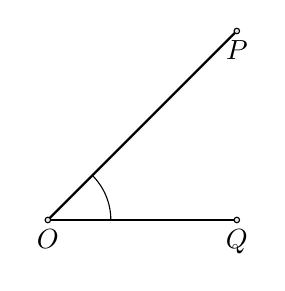
\begin{tikzpicture}[scale=.8]

% definitions
\tkzDefPoint(0,0){O}
\tkzDefPoint(3,3){P}
\tkzDefPoint(3,0){Q}
\tkzMarkAngle[label=QOP, size=1](Q,O,P)

\tkzDrawSegments[thick](O,P)
\tkzDrawSegments[thick](O,Q)
\tkzDrawPoints(O,P,Q)

% labels
\tkzLabelPoints(Q,O,P)
\end{tikzpicture}

$\angle{QOP} < 0$  o $\angle{QOP} > 12:00:00h $ (los angulos mayores de 180 grados se representan con valor negativo)
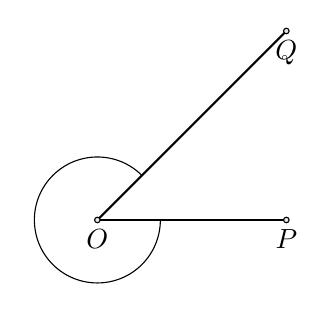
\begin{tikzpicture}[scale=.8]

% definitions
\tkzDefPoint(0,0){O}
\tkzDefPoint(3,3){Q}
\tkzDefPoint(3,0){P}
\tkzMarkAngle[label=QOP, size=1](Q,O,P)

\tkzDrawSegments[thick](O,P)
\tkzDrawSegments[thick](O,Q)
\tkzDrawPoints(O,P,Q)

% labels
\tkzLabelPoints(Q,O,P)
\end{tikzpicture}



\begin{itemize}
\item O: centro de la tierra y de la esfera celeste (esfera que contiene la esfera de la tierra, el plano ecuadorial terrestre se extiende al plano ecuadorial celeste y la comparte igual que la tierra en 2 hemisferios: norte y sur y el plano del meridiano 0 se puede extender para toda la esfera celeste). La correspondiente de la latitud en la tierra es la declinación para la esfera celeste (negativa si el objeto a observar está en hemisferio sur celeste) y para la longitud la declinación recta(positiva desde el meridiano 0 en el sentido de la rotación dela tierra en torno a su propio eje y negativa en el otro sentido)
\item P: punto del observador
\item T: posicion del objeto observado
\end{itemize}

Proyeccion longitudinal
P está en el hemisferio norte(latitud positiva) 
\vspace{5cm}


Declinacion negativa
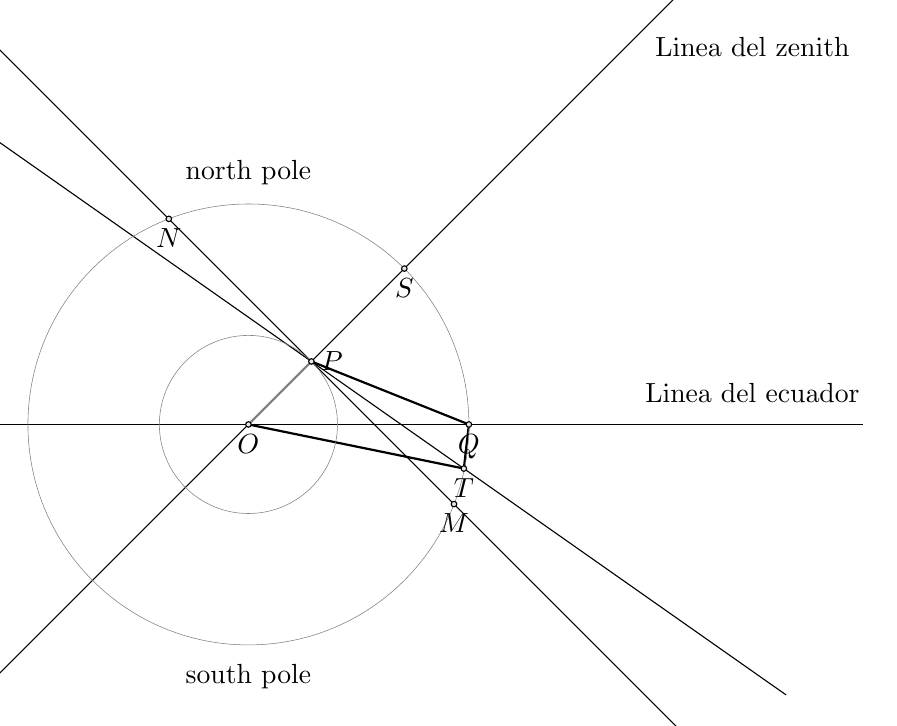
\begin{tikzpicture}[scale=.8]

% definitions
\tkzDefPoint(0,0){O}
\tkzDefPoint(1,1){P}
\tkzDefPoint(3.5,0){Q}
\tkzDefPoint(3.42,-0.7){T}

\tkzDefPointWith[orthogonal](P,O) \tkzGetPoint{P1} % find a point P1 orthogonal to PO
\tkzInterLC(P,P1)(O,Q) \tkzGetPoints{M}{N} % find intersections of a line passing through A and Q with the large circle 
\tkzInterLC(O,P)(O,Q) \tkzGetPoints{P4}{S} % find intersections of a line passing through A and Q with the large circle 
\draw [shorten >= -5cm, shorten <=-5cm] (P4)--(S);
\draw [shorten >= -5cm, shorten <=-5cm] (O)--(Q);
\node at (8,0.5){Linea del ecuador} ; 
\node at (8,6){Linea del zenith} ; 
\draw [shorten >= -5cm, shorten <=-5cm] (P)--(T) ;
\draw [shorten >= -5cm, shorten <=-5cm] (M)--(N) ;
%\tkzMarkAngle[label=lat, size=1](Q,O,P)

\tkzDrawSegments[thick](O,T)
\tkzDrawSegments[thick](T,Q)
\tkzDrawSegments[thick](P,Q)
%\tkzMarkAngle[](Q,O,T)
%\tkzMarkAngle[label=dec, size=1](Q,P,T)
%\tkzMarkAngle[label=zd, size=1](P4,P,T)
% drawing
\tkzDrawCircle(O,P)
\tkzDrawCircle(O,Q) 
\node at (0,4){north pole};
\node at (0,-4){south pole};
\tkzDrawSegments[thick,gray](O,P)
\tkzDrawPoints(O,P,Q,T,M,S,N)

% labels
\tkzLabelPoints(Q,T,O,M,S,N)
\tkzLabelPoints[right](P)
\end{tikzpicture}

\vspace{5cm}

Declinacion positiva
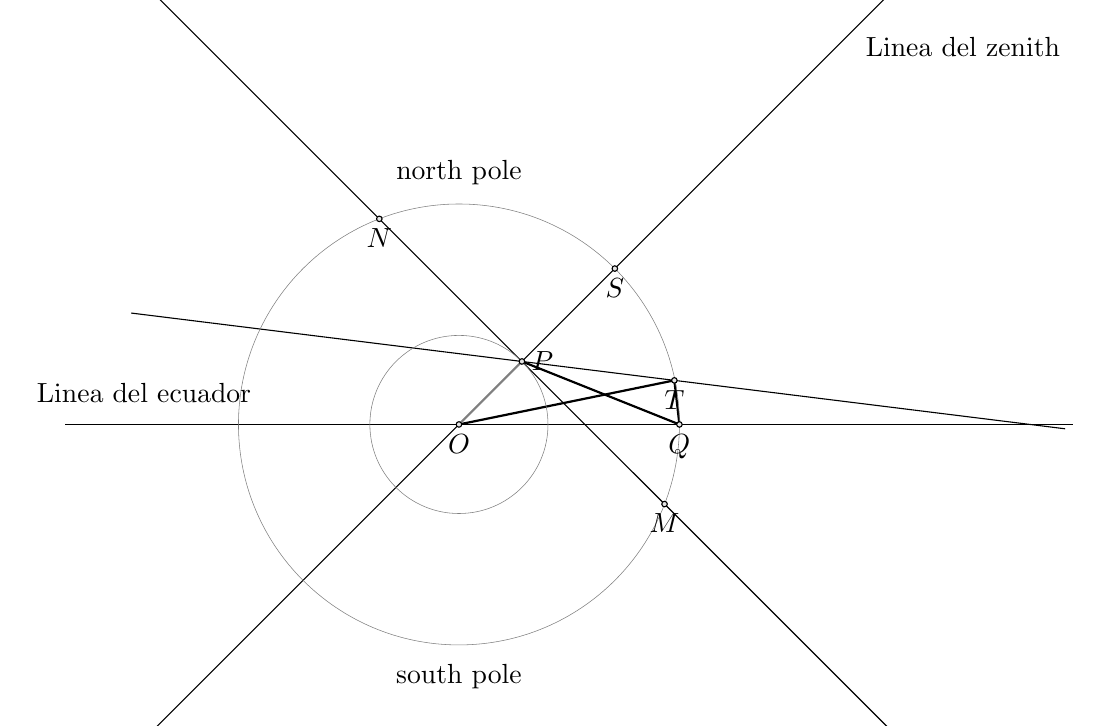
\begin{tikzpicture}[scale=.8]

% definitions
\tkzDefPoint(0,0){O}
\tkzDefPoint(1,1){P}
\tkzDefPoint(3.5,0){Q}
\tkzDefPoint(3.42,0.7){T}
\node at (-5,0.5){Linea del ecuador} ; 
\node at (8,6){Linea del zenith} ; 

\tkzDefPointWith[orthogonal](P,O) \tkzGetPoint{P1} % find a point P1 orthogonal to PO
\tkzInterLC(P,P1)(O,Q) \tkzGetPoints{M}{N} % find intersections of a line passing through A and Q with the large circle 
\tkzInterLC(O,P)(O,Q) \tkzGetPoints{P4}{S} % find intersections of a line passing through A and Q with the large circle 
\draw [shorten >= -5cm, shorten <=-5cm] (P4)--(S);
\draw [shorten >= -5cm, shorten <=-5cm] (O)--(Q) ;
\draw [shorten >= -5cm, shorten <=-5cm] (P)--(T) ;
\draw [shorten >= -5cm, shorten <=-5cm] (M)--(N) ;
%\tkzMarkAngle[label=lat, size=1](Q,O,P)

\tkzDrawSegments[thick](O,T)
\tkzDrawSegments[thick](T,Q)
\tkzDrawSegments[thick](P,Q)
%\tkzMarkAngle[](Q,O,T)
%\tkzMarkAngle[label=dec, size=1](Q,P,T)
%\tkzMarkAngle[label=zd, size=1](P4,P,T)
% drawing
\tkzDrawCircle(O,P)
\tkzDrawCircle(O,Q)
\node at (0,4){north pole};
\node at (0,-4){south pole};
\tkzDrawSegments[thick,gray](O,P)
\tkzDrawPoints(O,P,Q,T,M,S,N)

% labels
\tkzLabelPoints(Q,T,O,M,S,N)
\tkzLabelPoints[right](P)
\end{tikzpicture}


\vspace{5cm}
\begin{itemize}
\item OQ: linea del ecuador
\item OP: linea del zenit del observador(la linea que une el observador con el centro de la tierra) perpendicular en la linea del horizonte MN(solo se pueden ver objetos en el arco MSN: objetos con declinación entre -(90$^\circ$ - latitude) y 180$^\circ$ - (90$^\circ$ - latitude) )
\item PT: linea de vision del observador
\item $\angle{QPT}$ Para la proyeccion longitudinal es declinacion medida por el telescopio(negativa si la estrella está debajo del plano ecuadorial) - el angulo en el cielo entre la dirección del telescopio orientado hacia el objeto que observamos y la direccion del telescopio orientado hacía un objeto que está en el ecuador celeste. 
\item $\angle{QOT}$  declinacion  de la estrella (negativa si la estrella está debajo del plano ecuadorial) - medida desde un punto que esta en el ecuador de la tierra 
\item $\angle{QOP}$  latitud
\item $\angle{TPS}$  proyeccion en este plan del angulo zenith distance(formado por la linea del zenith y la direccion en cual apunta el telescopio) 
\item En práctica esta es zenith distance (el azimuth no cuenta) ZD medida en grados  (dd:mm:ss) con dd entre 00 y 90
y Airmass se aproxima como 1 / cos(ZD)


\end{itemize}
\begin{description}
\item $\angle{POQ} = \angle{POT} + \angle{TOQ}$
\item Q(el objeto de referrencia) está muy lejos asi que las distancias $OQ, PQ, PT, OT \gg OP$(el radio de la tierra) y  $\angle{TPQ}\approx \angle{TOQ} $ (la declinacion medida por el telescopio es aprox la declinacion del objeto observado medida desde un punto del ecuador terrestre si el objeto está bastante lejos)  	
\item Ademas si se apunta el telescopio cerca al zenith $\angle{SPT} \approx \angle{POT} \approx 0$ así que $\angle{POQ} \approx \angle{TPQ}$(latitud $\approx$ declinación)
\item Miramos las imagenes del flat del cielo (cuando el telescopio esta orientado aprox hacia el zenith) y determinamos la latitud 28:17:48
(grados)
\end{description}

Proyeccion transversal
P está al este del meridiano 0 terrestre(longitud positiva)

\vspace{5cm}

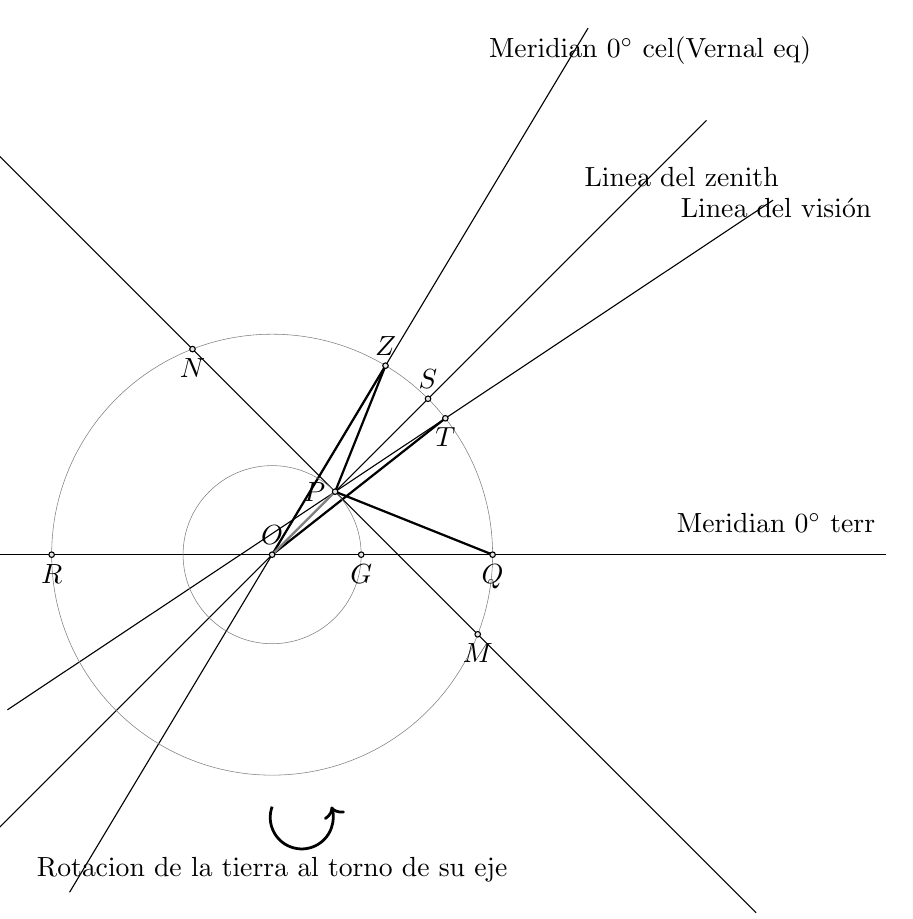
\begin{tikzpicture}[scale=.8]

% definitions
\tkzDefPoint(0,0){O}
\tkzDefPoint(1,1){P}
\tkzDefPoint(3.5,0){Q}
\tkzDefPoint(-3.5,0){R}
\tkzDefPoint(2.75,2.165){T}
\tkzDefPoint(1.8, 3){Z}
\node at (8,0.5){Meridian 0$^\circ$ terr} ; 
\node at (6,8){Meridian 0$^\circ$ cel(Vernal eq)} ; 
\node at (6.5,6){Linea del zenith} ; 
\node at (8,5.5){Linea del visión} ; 

\tkzDefPointWith[orthogonal](P,O) \tkzGetPoint{P1} % find a point P1 orthogonal to PO
\tkzInterLC(P,P1)(O,Q) \tkzGetPoints{M}{N} % find intersections of a line passing through A and Q with the large circle 
\tkzInterLC(O,P)(O,Q) \tkzGetPoints{P4}{S} % find intersections of a line passing through A and Q with the large circle 
\tkzInterLC(Q,R)(O,P) \tkzGetPoints{G}{P5} % find intersections of a line passing through A and Q with the large circle 
\draw [shorten >= -5cm, shorten <=-5cm] (P4)--(S);
\draw [shorten >= -5cm, shorten <=-5cm] (O)--(Q) ;
\draw [shorten >= -5cm, shorten <=-5cm] (O)--(Z) ;
\draw [shorten >= -5cm, shorten <=-5cm] (P)--(T) ;
\draw [shorten >= -5cm, shorten <=-5cm] (M)--(N) ;
%\tkzMarkAngle[label=lat, size=1](Q,O,P)

%\tkzDrawSegments[thick](O,T)
%\tkzDrawSegments[thick](T,Q)
\tkzDrawSegments[thick](P,Q)
\tkzDrawSegments[thick](P,Z)
\tkzDrawSegments[thick](O,Z)
\tkzDrawSegments[thick](O,T)
%\tkzMarkAngle[](Q,O,T)
%\tkzMarkAngle[label=dec, size=1](Q,P,T)
%\tkzMarkAngle[label=zd, size=1](P4,P,T)
% drawing
\tkzDrawCircle(O,P)
\tkzDrawCircle(O,Q)
\draw [->,line width=1pt] (0,-4) arc[x radius=0.5cm, y radius =.5cm, start angle=-200, end angle=20];
\node at (0,-5){Rotacion de la tierra al torno de su eje} ; 
\tkzDrawSegments[thick,gray](O,P)
\tkzDrawPoints(O,P,Q,T,M,S,N,Z,R,G)

% labels
\tkzLabelPoints(Q,T,M,N,R,G)
\tkzLabelPoints[left](P)
\tkzLabelPoints[above](O,Z,S)
\end{tikzpicture}

\vspace{5cm}
\begin{itemize}
\item Z vernal equinox
\item G punto en la tierra en el meridiano 0
\item $\angle{ZOQ}$ UniversalTime
\item $\angle{ZPT} \approx \angle{ZOT}$ RightAscension
\item $\angle{ZPS} \approx \angle{ZOS}$ SiderealTime
\item $\angle{SPT} \approx \angle{SOT}$ object hour
\item (ST = RA + h), cuando el objeto a observar está justo arriba(h=0) ST = RA
\item $\angle{QOP}$ longitud
\end{itemize}


\begin{description}
\item Cuando Sidereal Time es aprox 0 UT representa la longitud
\item longitud 22:21:45(hours) = -24:34:45(degrees)    

\end{description}


\end{document}
